\documentclass[conference]{IEEEtran}
\IEEEoverridecommandlockouts

\usepackage{cite}
\usepackage{amsmath,amssymb,amsfonts}
\usepackage{graphicx}
\usepackage{textcomp}
\usepackage{xcolor}
\usepackage{booktabs}
\usepackage{float}
\usepackage{array}
\usepackage[hidelinks]{hyperref}
\usepackage{url}

\def\BibTeX{{\rm B\kern-.05em{\sc i\kern-.025em b}\kern-.08em
    T\kern-.1667em\lower.7ex\hbox{E}\kern-.125emX}}

\begin{document}

\title{Distributed Analysis and Predictive Modelling of Short-Term Rentals: A PySpark Pipeline Over Porto, Lisbon, Madrid and Barcelona Airbnb Data\\
{\footnotesize \textsuperscript{*}Big Data Engineering (EGD), MECD, FEUP}}

\author{
    \IEEEauthorblockN{Daniel Dória}
    \IEEEauthorblockA{\textit{MECD} \\
    \textit{Faculty of Engineering, UP}\\
    Porto, Portugal \\
    up202108808@up.pt}
    \and
    \IEEEauthorblockN{Diego Montoya}
    \IEEEauthorblockA{\textit{MECD} \\
    \textit{Faculty of Engineering, UP}\\
    Porto, Portugal \\
    up202502851@up.pt}
    \and
    \IEEEauthorblockN{Jorge Gamonal}
    \IEEEauthorblockA{\textit{MECD} \\
    \textit{Faculty of Engineering, UP}\\
    Porto, Portugal \\
    up202602660@up.pt}
    \and
    \IEEEauthorblockN{José Evans}
    \IEEEauthorblockA{\textit{MECD} \\
    \textit{Faculty of Engineering, UP}\\
    Porto, Portugal \\
    up202108818@up.pt}
    \and
    \IEEEauthorblockN{Miguel Santos}
    \IEEEauthorblockA{\textit{MECD} \\
    \textit{Faculty of Engineering, UP}\\
    Porto, Portugal \\
    up202008450@up.pt}
}


\maketitle

\begin{abstract}
We present an end-to-end Big Data pipeline for the analytical exploration and predictive modelling of Inside Airbnb short-term-rental data covering four major Iberian cities (Porto, Lisbon, Madrid and Barcelona) on Apache Spark. The pipeline ingests 68{,}521 listings, a 25.8\,M-row daily availability calendar and 4.90\,M reviews from raw CSV into Parquet, executes eleven cross-city analytical queries, and trains three machine-learning models on a shared, leakage-safe MLlib feature pipeline. A gradient-boosted price regressor attains $R^2_{\log} = 0.72$ ($\text{RMSE} = \text{\texteuro}78$) on the held-out test split; a random forest predicts a listing's long-run high-occupancy status with $\text{AUC}=0.73$; and a month-aware classifier on a 684\,K-row calendar--listings panel predicts high-demand months with $\text{AUC}=0.77$ using a cyclic encoding of the calendar month. A scalability study on Google Dataproc benchmarks five workloads across 1, 2 and 4 worker nodes: join-heavy workloads gain up to $S(2)=1.98$ from one to two nodes, with diminishing returns beyond, as fixed overheads come to dominate at this data scale.
\end{abstract}

\begin{IEEEkeywords}
Apache Spark, MLlib, distributed computing, Airbnb, price prediction, occupancy forecasting, big data engineering
\end{IEEEkeywords}

% ─────────────────────────────────────────────────────────────────────────────
\section{Introduction}

The short-term rental sector has become a major component of urban tourism, with platforms such as Airbnb listing millions of properties worldwide. The Inside Airbnb project~\cite{insideairbnb2024} publicly scrapes per-city snapshots of listings, availability calendars and reviews, producing a large, heterogeneous dataset that has fuelled both academic research and policy debate.

Even at the scale of four medium-to-large European cities, the data is non-trivial: our combined snapshot contains 25.8\,M calendar rows and 4.90\,M reviews. Single-machine workflows struggle with this volume, motivating a Spark-based distributed pipeline. This work makes four contributions:
\begin{enumerate}
  \item A reproducible PySpark pipeline (ingest~$\to$~clean~$\to$~query~$\to$~model) operating over Porto, Lisbon, Madrid and Barcelona;
  \item Eleven analytical queries materialised as Parquet artefacts, spanning cross-city price, host-concentration and seasonality analyses;
  \item Three machine-learning models on a shared, leakage-safe MLlib feature pipeline: price regression, annual occupancy classification, and a month-aware occupancy classifier trained on the calendar~$\times$~listings join;
  \item A multi-node scalability study on Google Dataproc, benchmarking five representative workloads across 1, 2 and 4 worker nodes.
\end{enumerate}

% ─────────────────────────────────────────────────────────────────────────────
\section{Related Work}

\subsection{Airbnb price prediction}
Hedonic-pricing models are the long-standing baseline for short-term-rental valuation. Wang and Nicolau~\cite{wang2017price} fit a hedonic model on a 33-city Airbnb panel and showed that location, host attributes, room type and amenities together account for roughly 40\% of price variance. Chen and Xie~\cite{chen2017consumer} applied a similar framework to Austin listings, isolating a significant effect for professionally managed multi-listing hosts; the host's listing count is likewise among the most important price features in our model (Section~\ref{sec:importance}).

Machine-learning approaches push accuracy higher. Kalehbasti et al.~\cite{kalehbasti2019airbnb} combined gradient boosting with review-sentiment analysis on New York City data and report $R^2 \approx 0.69$ on log-price. Tang and Sangani~\cite{tang2015neighborhood} earlier achieved $R^2 \approx 0.65$ on San Francisco data using support-vector regression over a comparable feature set. Our gradient-boosted model reaches $R^2_{\log} = 0.715$ across the four Iberian cities using only the structural features that Inside Airbnb publishes (no listing text or review sentiment), suggesting that careful encoding of high-cardinality categorical variables can partially substitute for textual features.

\subsection{Demand and occupancy forecasting}
Hotel demand forecasting has a long pedigree~\cite{yang2014predicting,pan2012forecasting}, with recent work~\cite{cai2019hotel} layering deep-learning hybrids on classical ARIMA. The Airbnb-specific literature on occupancy prediction is comparatively sparse, with most studies focusing on price or growth. Our month-aware classifier targets this gap, using the daily availability calendar as the demand signal. We adopt the cyclic month encoding $(\sin(2\pi m/12), \cos(2\pi m/12))$ of Liu and Wang~\cite{liu2018cyclic}, which preserves the adjacency of December and January.

\subsection{Big-data engineering and Iberian context}
Apache Spark~\cite{zaharia2016apache} is the foundational engine for our distributed processing; we make extensive use of MLlib's Pipeline API~\cite{meng2016mllib}, in particular the standard \texttt{StringIndexer} $\to$ \texttt{OneHot\-Encoder} $\to$ \texttt{Vector\-Assembler} $\to$ \texttt{Standard\-Scaler} sequence. For the high-cardinality neighbourhood field we apply Micci-Barreca's target encoding~\cite{miccibarreca2001preprocessing}, computing the per-neighbourhood mean log-price on the training split only to prevent leakage. The Iberian context is documented by Guti{\'e}rrez et al.~\cite{gutierrez2017eruption} (Barcelona) and Cocola-Gant~\cite{cocolagant2018tourism} (Lisbon tourism gentrification), both of which highlight the spatial concentration patterns we observe. For the tree ensembles we rely on the canonical foundations of Random Forests~\cite{breiman2001random} and gradient boosting~\cite{friedman2001greedy}, as implemented in MLlib.

% ─────────────────────────────────────────────────────────────────────────────
\section{Data and Preparation}

\subsection{Data sources}
We use Inside Airbnb snapshots for each city. Two CSV variants are joined on listing identifier: a \emph{summary} file (18 columns; clean structural fields, integer prices) and a \emph{detailed} file (79 columns; richer structural, host and review attributes, with a dollar-formatted price). The principal fields used throughout this study are catalogued in Table~\ref{tab:dict}. In the summary file the nightly price is missing for a sizeable share of rows (from $\approx 11\%$ in Porto to $\approx 24\%$ in Madrid, about $18\%$ overall), so the cleaning stage coalesces the two price sources, preferring the detailed value where available, to maximise coverage.

\begin{table*}[t]
\caption{Data dictionary: principal fields used in the analysis and models}
\label{tab:dict}
\centering
\footnotesize
\begin{tabular}{@{}l l@{}}
\toprule
\textbf{Field} & \textbf{Description} \\
\midrule
\multicolumn{2}{@{}l}{\textit{Structural and capacity}}\\
\texttt{accommodates}                       & Guest capacity (number of guests the listing sleeps) \\
\texttt{bedrooms}, \texttt{beds}, \texttt{bathrooms} & Room, bed and bathroom counts \\
\texttt{property\_type}                     & Dwelling type (entire apartment, house, etc.) \\
\texttt{room\_type}                         & Entire home / private room / hotel room / shared room \\
\texttt{amenity\_count}                     & Number of amenities listed (derived from the amenities array) \\
\texttt{minimum\_nights}                    & Minimum nights required per booking \\
\addlinespace
\multicolumn{2}{@{}l}{\textit{Location}}\\
\texttt{latitude}, \texttt{longitude}       & Geographic coordinates \\
\texttt{neighbourhood}                      & Cleansed neighbourhood name (483 distinct across the four cities) \\
\texttt{neighbourhood\_group}               & Higher-level grouping: district (Spanish cities) or municipality (Portuguese cities) \\
\addlinespace
\multicolumn{2}{@{}l}{\textit{Host}}\\
\texttt{calculated\_host\_listings\_count}  & Number of active listings managed by the host \\
\texttt{host\_is\_superhost}                & Airbnb ``superhost'' status flag \\
\addlinespace
\multicolumn{2}{@{}l}{\textit{Reviews and activity}}\\
\texttt{number\_of\_reviews}, \texttt{number\_of\_reviews\_ltm} & Lifetime and last-12-month review counts \\
\texttt{reviews\_per\_month}                & Average monthly review rate \\
\texttt{review\_scores\_*}                  & Guest rating sub-scores (overall, cleanliness, location, value) \\
\addlinespace
\multicolumn{2}{@{}l}{\textit{Price and availability}}\\
\texttt{price}                             & Nightly price in \texteuro\ (source of the regression target) \\
\texttt{availability\_365}                  & Bookable days over the next year \\
\texttt{occupancy\_rate}                     & $1 - \texttt{availability\_365}/365$, used as an annual demand proxy \\
\addlinespace
\multicolumn{2}{@{}l}{\textit{Engineered for modelling (Section~\ref{sec:ml})}}\\
\texttt{neighbourhood\_mean\_log\_price}    & Target encoding: mean training log-price of the neighbourhood \\
\texttt{log\_reviews}, \texttt{log\_host\_listings} & Log-transformed skewed counts \\
\texttt{recent\_activity\_ratio}            & Share of a listing's reviews received in the last 12 months \\
\texttt{min\_nights\_cat}                   & Bucketed minimum-nights category \\
\bottomrule
\end{tabular}
\end{table*}

\subsection{Cleaning and statistics}
After casting the dollar-formatted price to a numeric type, dropping rows with null or zero price, deduplicating by listing identifier, and joining the detailed file, we obtain 68{,}521 listings. Table~\ref{tab:dataset} summarises the cleaned data per city: Lisbon and Madrid contribute the bulk of the inventory, Porto has the lowest median price and Barcelona the highest.

\begin{table}[H]
\caption{Cleaned dataset statistics per city}
\label{tab:dataset}
\centering
\begin{tabular}{lrrrr}
\toprule
\textbf{City} & \textbf{Listings} & \textbf{Median \texteuro} & \textbf{Calendar} & \textbf{Reviews} \\
\midrule
Porto     & 13{,}189 & 90  & 5.43\,M  & 1.00\,M \\
Lisbon    & 21{,}466 & 109 & 8.98\,M  & 1.68\,M \\
Madrid    & 18{,}953 & 110 & 9.13\,M  & 1.27\,M \\
Barcelona & 14{,}913 & 143 & 2.30\,M  & 0.95\,M \\
\midrule
Total     & 68{,}521 & --- & 25.84\,M & 4.90\,M \\
\bottomrule
\end{tabular}
\end{table}

\subsection{Storage and partitioning}
All processed tables are written as Snappy-compressed Parquet, partitioned by city (Hive-style, e.g.\ \texttt{listings/city=porto/}). Partitioning enables partition pruning during single-city queries and parallel reads across partitions for cross-city operations, and it is the physical layout the scalability study (Section~\ref{sec:perf}) exercises.

\subsection{Exploratory findings}
Three descriptive patterns emerge from initial profiling. First, the median nightly price is highest in Barcelona (\texteuro143), comparable in Lisbon (\texteuro109) and Madrid (\texteuro110), and materially lower in Porto (\texteuro90). Second, room-type composition is similar across the four cities, with entire homes or apartments dominating everywhere, from 71\% of listings in Barcelona to 84\% in Porto. Third, host concentration is high throughout: hosts with more than one listing hold between 75\% (Lisbon) and 81\% (Barcelona) of inventory, consistent with the professionalisation effect reported by Wang and Nicolau~\cite{wang2017price}.

% ─────────────────────────────────────────────────────────────────────────────
\section{Analytical Queries}

\subsection{Architecture}
Each query is implemented as a self-contained module exposing a uniform \mbox{$\texttt{run(spark)} \to \texttt{DataFrame}$} interface and registered in a central catalogue. A single driver job runs any query by identifier and persists its result to Parquet, decoupling computation from the downstream consumers (analysis notebooks, an interactive Streamlit dashboard, and this report).

\subsection{Query catalogue}
Table~\ref{tab:queries} lists all eleven queries. They span the three dataset types (listings, calendar, reviews) and cover both descriptive analytics (price distributions, host concentration) and joins of meaningful big-data scale: Q2 in particular joins the 25.8\,M-row calendar with the 68.5\,K-row listings table.

\begin{table}[H]
\caption{Analytical query catalogue}
\label{tab:queries}
\centering
\renewcommand{\arraystretch}{1.15}
\begin{tabular}{p{0.4cm}p{6.7cm}}
\toprule
\textbf{ID} & \textbf{Question / output} \\
\midrule
Q1  & Top and bottom 10 neighbourhoods by median price per city \\
Q2  & Monthly availability and occupancy (calendar $\times$ listings) \\
Q3  & Average availability and occupancy by room type $\times$ city \\
Q4  & Multi-listing vs.\ single-listing host comparison \\
Q5  & Host concentration (Pareto curve of listings per host) \\
Q6  & Pearson correlation: reviews/month $\times$ price per neighbourhood \\
Q7  & Top 10 neighbourhoods by estimated annual revenue \\
Q8  & Room-type market share per city \\
Q9  & Monthly review trend and year-over-year growth \\
Q10 & Price-outlier share (\texteuro{}100/\texteuro{}250/\texteuro{}500) per room type \\
Q11 & District/municipality comparison (higher-level grouping) \\
\bottomrule
\end{tabular}
\end{table}

\subsection{Selected findings}
Three queries illustrate the cross-city patterns this analysis surfaces. \textbf{Q5} confirms a heavy Pareto distribution of inventory (Fig.~\ref{fig:pareto}): the top decile of hosts holds essentially half of all listings in Porto and Lisbon ($49\%$ in both), rising to $56\%$ in Madrid and $59\%$ in Barcelona; in every city the curve sits well above the equal-share diagonal.

\textbf{Q2} reveals heterogeneous monthly demand (Fig.~\ref{fig:seasonality}). The three coastal-tourism cities peak in June--July, with a June--August occupancy lift of $+34\%$ above the annual mean in Barcelona, $+39\%$ in Lisbon and $+61\%$ in Porto; inland Madrid carries only a mild summer lift ($+7\%$) and instead reaches its highest occupancy in September--October, consistent with a year-round business and city-break profile rather than a leisure-season one.

\textbf{Q11} shows that in the two Spanish cities a single central district dominates its city's inventory: Madrid's \emph{Centro} ($\approx 8.1$\,K listings) and Barcelona's \emph{Eixample} ($\approx 5.4$\,K), echoing the spatial concentration documented for Mediterranean tourism markets~\cite{gutierrez2017eruption}.

% ─────────────────────────────────────────────────────────────────────────────
\section{Machine-Learning Pipeline}
\label{sec:ml}

\subsection{Shared feature pipeline}
All three models share a single MLlib pipeline, parameterised by the target column and terminated by the model's estimator. The four preceding preprocessing stages are:
\begin{enumerate}
  \item \textbf{Feature engineering} --- derive seven columns: the annual occupancy rate, log-transformed review and host-listing counts, a recent-activity ratio, a bucketed minimum-nights category, and the two-column neighbourhood target encoding (Table~\ref{tab:dict});
  \item \textbf{Selection and imputation} --- project to the model columns and impute missing structural fields (bedrooms, ratings, etc.) with sensible defaults;
  \item \texttt{StringIndexer} $\to$ \texttt{OneHotEncoder} on the categorical features;
  \item \texttt{VectorAssembler} $\to$ \texttt{StandardScaler} (without centring: trees are scale-invariant, but linear regression benefits from comparable feature scales).
\end{enumerate}

\begin{figure}[tb]
\centering
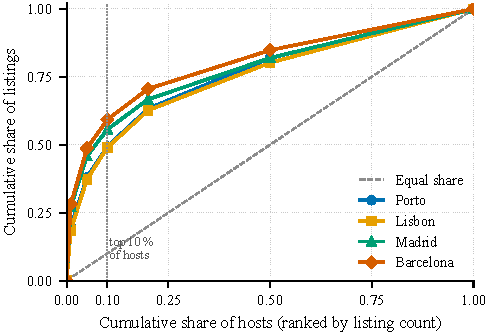
\includegraphics[width=\columnwidth]{../figures/host_pareto.pdf}
\caption{Host-concentration Pareto curves per city: cumulative share of listings held by the top fraction of hosts (ranked by listing count). The dashed diagonal is the equal-share reference. The dotted vertical line marks the top-decile of hosts referenced in the text (49--59\% of inventory across the four cities).}
\label{fig:pareto}
\end{figure}

\begin{figure}[tb]
\centering
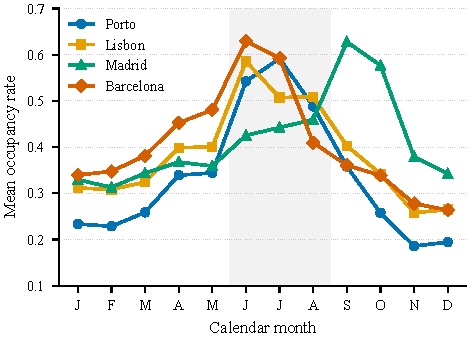
\includegraphics[width=\columnwidth]{../figures/seasonality_by_city.pdf}
\caption{Monthly occupancy rate per city, averaged across the available calendar window (Q2). The shaded band marks June--August. Porto, Lisbon and Barcelona peak inside this window; Madrid's peak instead falls in September--October, a structurally different seasonality.}
\label{fig:seasonality}
\end{figure}

\textbf{Target encoding for high-cardinality categoricals.}
The neighbourhood field has 483 distinct values across the four cities --- too many for efficient one-hot encoding. Following Micci-Barreca~\cite{miccibarreca2001preprocessing}, we replace it with the mean $\log(1+\text{price})$ of training listings in that neighbourhood. These statistics are computed on the training split only, preventing target leakage.

\subsection{Price regression}
The target is $y = \log(1 + \text{price})$. A dynamic cap at the 99th percentile ($p_{99} = \text{\texteuro}1003$) removes high-end outliers that disproportionately inflate the squared-error loss. Three estimators are trained on an 80/20 split (seed 42):
\begin{itemize}
  \item \textbf{Ridge Linear Regression} --- $L_2$ regularisation, \mbox{$\lambda=0.01$};
  \item \textbf{Random Forest} --- 100 trees, depth 8, minimum 10 instances per node;
  \item \textbf{Gradient-Boosted Trees} --- 200 iterations, depth 6, step size 0.05, subsample rate 0.8.
\end{itemize}

Table~\ref{tab:price_results} reports both log-scale and back-transformed Euro-scale metrics. The gap between $R^2_{\log}$ and $R^2_{\text{\texteuro}}$ reflects the outlier-sensitivity of the squared error after exponentiation: small errors in log-space become large absolute errors at the top of the price distribution.

\begin{table}[H]
\caption{Price-regression results on the held-out test set ($n=13{,}341$)}
\label{tab:price_results}
\centering
\begin{tabular}{lcccccc}
\toprule
        & \multicolumn{3}{c}{\textbf{Log-scale}} & \multicolumn{3}{c}{\textbf{Euro-scale}} \\
\cmidrule(lr){2-4}\cmidrule(lr){5-7}
\textbf{Model} & RMSE & MAE & $R^2$ & RMSE & MAE & $R^2$ \\
\midrule
LR (ridge) & 0.430 & 0.319 & 0.617 & 87.3 & 46.2 & 0.473 \\
RF         & 0.408 & 0.302 & 0.655 & 86.4 & 44.6 & 0.484 \\
GBT        & \textbf{0.370} & \textbf{0.267} & \textbf{0.715} & \textbf{77.9} & \textbf{39.7} & \textbf{0.581} \\
\bottomrule
\end{tabular}
\end{table}

\subsection{Annual occupancy classifier}
A listing is labelled \emph{high-occupancy} when its booked fraction, $1 - \texttt{availability\_365}/365$, exceeds $0.70$. To prevent leakage, all availability-derived fields --- including the occupancy rate and the booked-night and revenue quantities computed from them --- are excluded from the feature set. The base rate on the training data is 21\%, so the classifiers use inverse-frequency class weighting. A random forest (150 trees, depth 12) achieves $\text{AUC}=0.73$ and $F_1=0.74$; logistic regression sits noticeably lower at $\text{AUC}=0.64$. The gap reflects the importance of non-linear interactions between location, room type and host professionalism.

\subsection{Month-aware occupancy classifier}
The third model joins the daily calendar with the listings table to construct a (listing, year, month) panel of approximately 684{,}000 observations. A monthly observation is retained only where at least 20 calendar days are available, and the target marks months whose occupancy rate exceeds $0.50$, a threshold chosen so the base rate is balanced at 37\% rather than the much lower long-run annual base rate.

The model adds three temporal features to the shared pipeline: the month index $m \in \{1,\dots,12\}$ and its cyclic pair $\sin(2\pi m/12)$, $\cos(2\pi m/12)$. The trigonometric encoding makes the model treat December and January as adjacent, which an ordinal index would not. A random forest then achieves $\text{AUC}=0.77$ on the held-out 136{,}773-row test set. This is not directly comparable with the annual classifier's $0.73$, since the two models target different occupancy thresholds (0.50 vs 0.70) on different units (listing-month panel vs listing), but it does show that high-demand months are learnable from a listing's structural features combined with a cyclic month encoding.

\subsection{Feature importance}
\label{sec:importance}
Table~\ref{tab:importance} lists the ten most important features for the GBT price model, aggregating the one-hot expansions of categorical features back to their parent column. The ranking aligns with the hedonic-pricing literature~\cite{wang2017price,chen2017consumer}: capacity and structural attributes (guest capacity, property and room type, amenity count), location (the neighbourhood target encoding, longitude, the district grouping) and host professionalism (the host's listing count) dominate. The superhost flag and the log-transformed host/review counts carried zero importance, and instant-bookability was negligible ($<0.2\%$); these were dropped from the operational dashboard's inputs.

\begin{table}[H]
\caption{Top-10 features by importance, GBT price model}
\label{tab:importance}
\centering
\begin{tabular}{lr}
\toprule
\textbf{Feature} & \textbf{Importance} \\
\midrule
\texttt{accommodates}                         & 0.106 \\
\texttt{property\_type}                       & 0.094 \\
\texttt{neighbourhood\_mean\_log\_price}      & 0.070 \\
\texttt{calculated\_host\_listings\_count}    & 0.065 \\
\texttt{minimum\_nights}                      & 0.051 \\
\texttt{room\_type}                           & 0.047 \\
\texttt{longitude}                            & 0.045 \\
\texttt{neighbourhood\_group}                 & 0.041 \\
\texttt{amenity\_count}                       & 0.039 \\
\texttt{review\_scores\_cleanliness}          & 0.037 \\
\bottomrule
\end{tabular}
\end{table}

% ─────────────────────────────────────────────────────────────────────────────
\section{Performance and Scalability}
\label{sec:perf}

To characterise how the pipeline scales with cluster size, we benchmark five representative workloads on Google Dataproc across 1, 2 and 4 worker nodes.

\subsection{Workloads}
The five workloads span the two dominant cost profiles in the pipeline, distributed shuffles and iterative ML training:
\begin{itemize}
  \item \textbf{Q2 seasonality} --- joins the 26\,M-row calendar with listings and aggregates to (city, year, month); shuffle-bound but emits only 53 rows;
  \item \textbf{Calendar revenue} --- the same join plus a per-month neighbourhood revenue aggregation and a windowed ranking;
  \item \textbf{Review demand} --- joins the 4.95\,M-row reviews table with listings and aggregates monthly review volume by price band, room type and city;
  \item \textbf{Full pipeline} --- a three-way calendar~$\times$~listings~$\times$~reviews join, the heaviest workload by wall-clock time;
  \item \textbf{RF price train} --- fits a representative random-forest price regressor (50 trees, depth 8) over the listings table; CPU- and memory-bound.
\end{itemize}

\subsection{Methodology and configuration}
Runs execute on Dataproc clusters of 1, 2 and 4 \texttt{n2-standard-4} workers (4 vCPUs / 16\,GB each; image 2.2-debian12, Spark 3.5), giving 4, 8 and 16 executor cores respectively. The benchmark reads a Google Cloud Storage copy of the four-city corpus in the same Snappy-Parquet layout (69{,}647 listings, 26.20\,M calendar rows and 4.95\,M reviews, within $\approx 2\%$ of Table~\ref{tab:dataset}; the small difference reflects a slightly earlier scrape). Each workload is timed three times per configuration with the Spark cache cleared between runs, and we report the median wall-clock time. The first run of every triple is a consistent cold-start outlier (roughly 2--3.5$\times$ slower) caused by executor JVM warm-up, broadcast and GCS metadata latency; being the slowest of the three, it is never selected as the median. Speedup is $S(n)=T(1)/T(n)$ and parallel efficiency $E(n)=S(n)/n$, both relative to the single-worker baseline.

\subsection{Results}
Table~\ref{tab:bench} and Fig.~\ref{fig:speedup} report the measurements.

\begin{table}[H]
\caption{Dataproc wall-clock seconds (median of 3 runs) and speedup relative to the 1-worker baseline}
\label{tab:bench}
\centering
\begin{tabular}{lrrrcc}
\toprule
 & \multicolumn{3}{c}{\textbf{Wall-clock (s)}} & \multicolumn{2}{c}{\textbf{Speedup}} \\
\cmidrule(lr){2-4}\cmidrule(lr){5-6}
\textbf{Workload} & 1w & 2w & 4w & $S(2)$ & $S(4)$ \\
\midrule
Q2 seasonality   & 22.4 & 22.5 & 17.1 & 1.00 & 1.31 \\
Calendar revenue & 26.5 & 16.6 & 17.4 & 1.59 & 1.53 \\
Review demand    & 36.9 & 18.7 & 15.5 & 1.98 & \textbf{2.39} \\
Full pipeline    & 40.2 & 22.9 & 22.7 & 1.75 & 1.77 \\
RF price train   & 60.5 & 39.7 & 40.6 & 1.53 & 1.49 \\
\bottomrule
\end{tabular}
\end{table}

\begin{figure}[H]
\centering
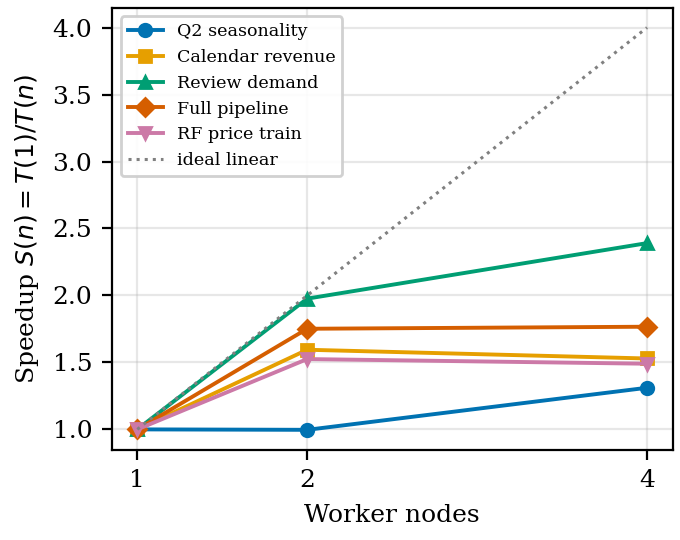
\includegraphics[width=0.92\columnwidth]{../figures/bench_speedup.png}
\caption{Speedup versus worker-node count on Dataproc. The heaviest shuffle (review demand) scales closest to linear; lighter workloads plateau after two workers.}
\label{fig:speedup}
\end{figure}

Three patterns emerge. First, scaling from one to two workers delivers most of the benefit: shuffle-heavy joins gain $S(2)\approx1.6$--$2.0$, with the heaviest workload (review demand, a 4.95\,M-row join) closest to linear at $S(2)=1.98$. Second, the step from two to four workers yields little further speedup: most workloads plateau ($S(4)\approx S(2)$) and parallel efficiency drops to $E(4)\approx0.33$--$0.60$. At these data volumes (tens of millions of rows; a few hundred MB of Parquet) a 16-core cluster is over-provisioned, so fixed per-stage overheads (task scheduling, shuffle setup, broadcast of the listings table, GCS I/O latency) dominate the shrinking per-core work. Third, the benefit tracks workload size: review demand and the full three-way join scale furthest, whereas Q2 seasonality --- which collapses 26\,M rows into a 53-row result --- barely benefits ($S(4)=1.31$) because its final aggregation is cheap and latency-bound. RF training is compute-bound and gains from the first doubling ($S(2)=1.53$) but not beyond, as the $\approx55$\,K-row training split is small relative to the broadcast and coordination cost of the growing ensemble.

The engineering lesson is consistent with distributed-computing theory: distribution pays off in proportion to shuffle and compute volume, and for this corpus two \texttt{n2-standard-4} workers already saturate the available parallelism. Sustained linear scaling to four nodes and beyond would require larger inputs (more cities or per-night granularity) or heavier models.

% ─────────────────────────────────────────────────────────────────────────────
\section{Discussion}

\textbf{Cross-city structure.} The clearest economic signal is a price gradient that tracks tourism intensity (Barcelona $>$ Madrid $\approx$ Lisbon $>$ Porto) and is only partly captured by the structural features in our model: the neighbourhood target encoding alone is the third most important GBT feature (Table~\ref{tab:importance}). Host concentration, by contrast, is strikingly uniform (75--81\% of inventory held by multi-listing operators), reinforcing the professionalisation thesis. Seasonality is the dimension that separates the markets most sharply, with a pronounced June--July peak in the coastal cities versus a delayed September--October peak in inland Madrid (Fig.~\ref{fig:seasonality}); both patterns are signals that the month-aware model exploits.

\textbf{Price model in context.} The GBT log-$R^2$ of $0.715$ marginally exceeds the $R^2 \approx 0.69$ of Kalehbasti et al.~\cite{kalehbasti2019airbnb} on New York and the $R^2 \approx 0.65$ of Tang and Sangani~\cite{tang2015neighborhood} on San Francisco, despite using only published structural features (no review text or sentiment). We attribute this partly to the target-encoded neighbourhood feature, which captures fine-grained location signal that one-hot encoding would dilute across 483 sparse columns. The Euro-scale RMSE of \texteuro78, against per-city medians in the \texteuro90--\texteuro143 range (Table~\ref{tab:dataset}), reflects the heavy right tail of the price distribution rather than systematic bias, since the log-scale fit is strong.

\textbf{Monthly demand.} The month-aware classifier reaches $\text{AUC}=0.77$ on a balanced (37\%) base rate; while the comparison with the annual model is informal (the two operate on different targets), the result confirms that monthly demand is learnable from listing structure combined with a cyclic month encoding.

\textbf{Limitations.} The snapshots contain nulls in the summary-format price (mitigated by the detailed-file join) and lack a usable adjusted price in the calendar, which precludes true per-night dynamic-pricing analysis. The Barcelona snapshot also carries a shorter forward calendar horizon than the other three cities (about 154 days per listing versus a full year); cross-city seasonality is therefore reported as occupancy \emph{rates} rather than raw day counts to remain comparable.

% ─────────────────────────────────────────────────────────────────────────────
\section{Reproducibility}

The pipeline is organised as a single repository in which the ingest, clean, query and training stages are exposed as command-line jobs and the generated artefacts (query results, trained model pipelines, feature importances and benchmark logs) are versioned alongside the code. All train/test splits use a fixed random seed (42). The software stack is Python~3.11 with PySpark~3.5 and MLlib; the cloud benchmark uses Dataproc image 2.2-debian12 and is driven by a standalone PySpark script together with the cluster-provisioning scripts in the repository. The four-city Inside Airbnb snapshots are public~\cite{insideairbnb2024}.

% ─────────────────────────────────────────────────────────────────────────────
\section{Conclusion}

We built and evaluated a complete distributed pipeline for short-term-rental analytics across Porto, Lisbon, Madrid and Barcelona: 68{,}521 listings, 25.8\,M calendar rows and 4.90\,M reviews ingested into Parquet, processed by eleven analytical queries, and modelled by three MLlib pipelines. The best price regressor (GBT) attains $R^2_{\log}=0.72$, $\text{RMSE}=\text{\texteuro}78$; the annual occupancy classifier reaches $\text{AUC}=0.73$, and a month-aware variant rises to $\text{AUC}=0.77$ on a 684\,K-row calendar panel. The Dataproc scalability study confirmed that the heavier shuffle workloads scale near-linearly to two worker nodes but plateau thereafter, the cluster being over-provisioned for this data volume.

Future work includes (i) integrating streaming calendar updates to enable dynamic price recommendation, (ii) extending the pipeline to further European cities for cross-market generalisation, and (iii) replacing manual hyperparameter choices with Spark \texttt{CrossValidator} grid search on the Dataproc cluster.

\bibliographystyle{IEEEtran}
\bibliography{references}

\end{document}
